\section{Analysis}

The results shown in this section are for gender prediction with ethnicity as protected group, and are summarized for all models below. The results for fair masking have $T_c = 0.1$.

\begin{table}[ht]
	\centering
	\begin{tabular}{ |c|c|c|c|c|c| } 
		\hline
		 Model & Training & Validation/Testing & Training & Validation & Unfairness \\
		  & accuracy (\%) & accuracy (\%) & loss & /Testing loss & \\
		 \hline
		 Logistic regression baseline & 73.51 & 72.97 &  0.0044 &  0.0045 & 0.0010\\
		 FeedForward baseline & 79.32 & 77.20 & 0.0066 & 0.0421 & 0.0015 \\
		 CNN baseline & 95.22 & 85.29 & 0.0009 & 0.0025 & 0.0012 \\
		 ResNet baseline & 97.93 & 86.71 & 0.0003 & 0.0035 & 0.0016 \\
		 Regularized ResNet & 98.26 & 88.03 & 0.0007 & 0.0074 & 0.0008 \\
		 Fair masking & 99.35 &  85.31 & 0.0001 & 0.0028 & 0.0011 \\
		 Transfer learning & N/A & 62.81 & N/A & 0.0103 & 0.0002 \\
		\hline
	\end{tabular}
	\caption{Training and validation accuracy and loss and unfairness measures of gender classification by model}
	\label{nnOA}
\end{table}

\begin{table}[ht]
	\centering
	\begin{tabular}{ |c|c|c|c|c|c|c|c| } 
		\hline
		 Model & Black & E. Asian & Indian & Latino & Mid. Eastern & S.E. Asian & White\\
		 
		 \hline
		 Logistic regression baseline & 67.35 & 72.26 &  74.74 &  75.97 & 77.58 & 71.52 & 72.37\\
		 FeedForward baseline & 74.17 & 78.18 & 81.84 & 81.97 &83.70&77.39&81.61\\
		 CNN baseline & 79.58&83.74&86.28&87.92&90.57&87.49&84.80 \\
		 ResNet baseline & 79.95&86.00&86.87&89.03&92.64&86.22&86.28\\
		 Regularized ResNet & 81.61&87.93&88.32&90.81&91.06&87.49&88.05 \\
		 Fair masking & 80.14&82.54&87.60&88.97&88.17&84.81&85.95 \\
		 Transfer learning & 63.14 &60.91 &62.49&65.54&64.83&62.85&62.60 \\
		\hline
	\end{tabular}
	\caption{Validation accuracy (\%) amongst ethnic groups for gender classification by model}
	\label{nnOA}
\end{table}

Note that, for all models aside from transfer learning, the evaluation accuracies are the lowest for the label "Black," which shows that the models are still somewhat unfair.

\newpage
\subsection{Non-deep learning baseline - Logistic Regression}
We use logistic regression for gender classification.   

\begin{figure}[H]
	\centering
	\begin{subfigure}
		\centering
		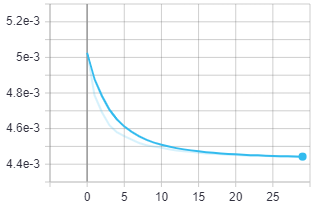
\includegraphics[width=0.4\textwidth]{figure/logistic-loss.png}
	\end{subfigure}
	\quad
	\begin{subfigure}
		\centering
		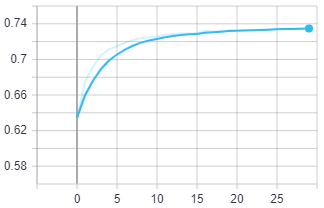
\includegraphics[width=0.4\textwidth]{figure/logistic-acc.png}
	\end{subfigure}
	\caption{Training loss and accuracy in gender classification for logistic baseline}
	\label{fig: logistic}
\end{figure}

\begin{itemize}
\item Training: final training accuracy and loss are 73.51\% and 0.0044, respectively.  

\item Validation: final validation accuracy and loss are 72.97\% and 0.0045, respectively.

\item UF for the validation set: unfairness parameter $UF$ in equation (1) on the validation set is 0.0010.   
\end{itemize}

\subsection{Deep learning baseline (1) - FeedForward Neural Network}

\begin{figure}[H]
	\centering
	\begin{subfigure}
		\centering
		\includegraphics[width=0.4\textwidth]{figure/feedforward_loss.PNG}
	\end{subfigure}
	\quad
	\begin{subfigure}
		\centering
		\includegraphics[width=0.4\textwidth]{figure/feedforward_acc.png}
	\end{subfigure}
	\caption{Training loss and accuracy in gender classification for CNN baseline.}
	\label{fig: feedforward}
\end{figure}

\begin{itemize}
\item Training: final training accuracy and loss are 79.32$\%$ and 0.0066, respectively.  

\item Validation: final validation accuracy and loss are 77.20$\%$ and 0.0421, respectively.

\item UF for the validation set: unfairness parameter on the validation set is 0.0015.   
\end{itemize}


\subsection{Deep learning baseline (2) - Convolutional Neural Network}

\begin{figure}[H]
	\centering
	\begin{subfigure}
		\centering
		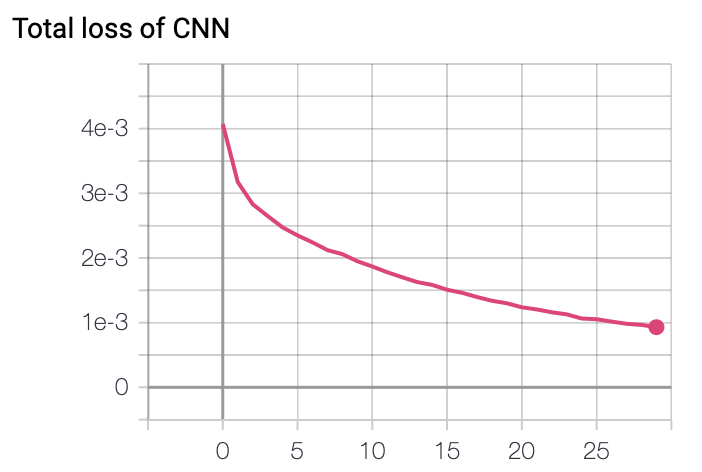
\includegraphics[width=0.4\textwidth]{figure/cnn-loss.png}
	\end{subfigure}
	\quad
	\begin{subfigure}
		\centering
		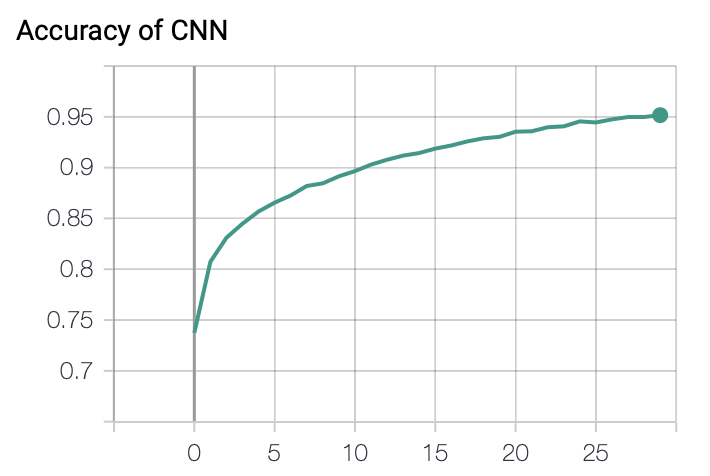
\includegraphics[width=0.4\textwidth]{figure/cnn-ac.png}
	\end{subfigure}
	\caption{Training loss and accuracy in gender classification for CNN baseline.}
	\label{fig: cnn}
\end{figure}

\begin{itemize}
\item Training: final training accuracy and loss are 95.22$\%$ and 0.0009, respectively.  

\item Validation: final validation accuracy and loss are 85.29$\%$ and 0.0025, respectively.

\item UF for the validation set: unfairness parameter on the validation set is 0.0012.   
\end{itemize}


\subsection{Deep learning baseline (3) - Residual Network}

\begin{figure}[H]
	\centering
	\begin{subfigure}
		\centering
		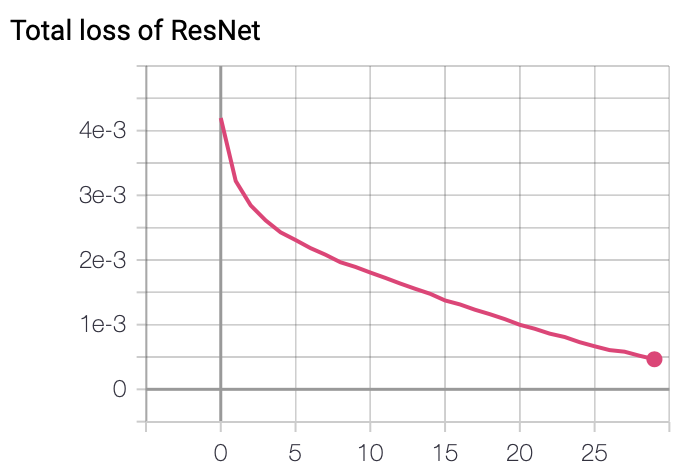
\includegraphics[width=0.4\textwidth]{figure/resnet-loss.png}
	\end{subfigure}
	\quad
	\begin{subfigure}
		\centering
		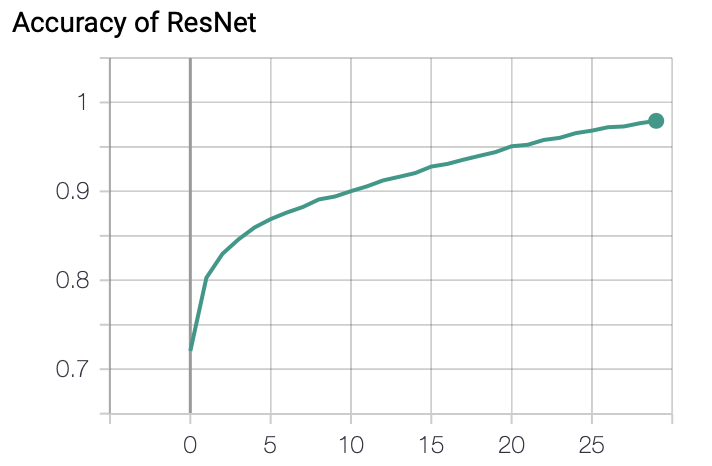
\includegraphics[width=0.4\textwidth]{figure/resnet-ac.png}
	\end{subfigure}
	\caption{Training loss and accuracy in gender classification for ResNet baseline.}
	\label{fig: resnet}
\end{figure}

\begin{itemize}
\item Training: final training accuracy and loss are 97.93$\%$ and 0.0003, respectively.  

\item Validation: final validation accuracy and loss are 86.71$\%$ and 0.0035, respectively.

\item UF for the validation set: unfairness parameter on the validation set is 0.0014.   
\end{itemize}


\subsection{Novel approach (1) - Regularized ResNet}

\begin{figure}[H]
	\centering
	\begin{subfigure}
		\centering
		\includegraphics[width=0.4\textwidth]{figure/res_pen_train.png}
	\end{subfigure}
	\quad
	\begin{subfigure}
		\centering
		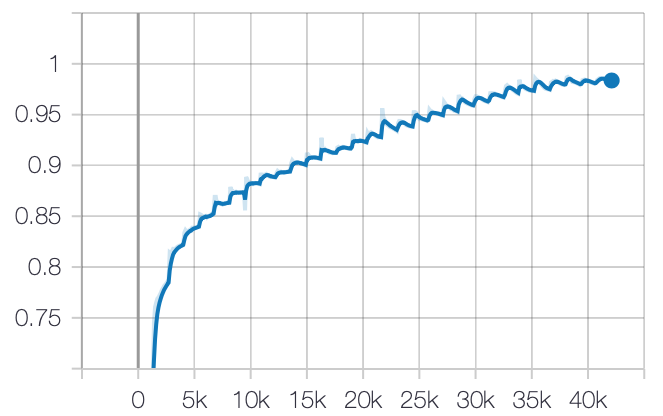
\includegraphics[width=0.4\textwidth]{figure/res_pen_acc.png}
	\end{subfigure}
	\caption{Training loss and accuracy in gender classification for regularized ResNet.}
	\label{fig: res pen}
\end{figure}

\begin{itemize}
\item Training: final training accuracy and loss are 98.26\% and 0.0007, respectively.

\item Validation: final validation accuracy and loss are 88.03\% and 0.0074, respectively.

\item UF for the validation set: unfairness parameter on the validation set is 0.0008.   
\end{itemize}

Note that the penalty is clearly applied, as the loss on the regularized ResNet is greater than that of the baseline ResNet. The UF value is significantly lower than those of the baseline models, confirming that our approach is effective with respect to improving fairness. However, we can see the accuracy of "Black" is still significantly lower than other ethnicity, which implies that we may need to use a lower weight in our penalty function, e.g. take $\frac{1}{10}*(acc_{black}-acc_{average})^2$. Due to time constraints, we were not able to test this, but it seems to be a promising direction for future work.

\subsection{Novel approach (2) - Fair Masking}

\begin{figure}[H]
	\centering
	\begin{subfigure}
		\centering
		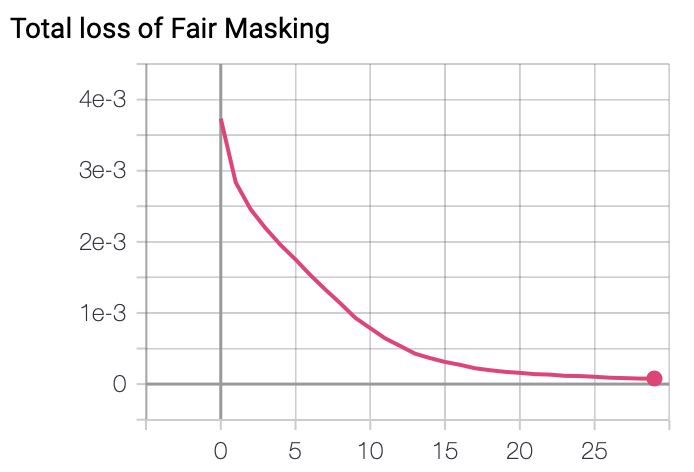
\includegraphics[width=0.4\textwidth]{figure/fairmasking-loss.png}
	\end{subfigure}
	\quad
	\begin{subfigure}
		\centering
		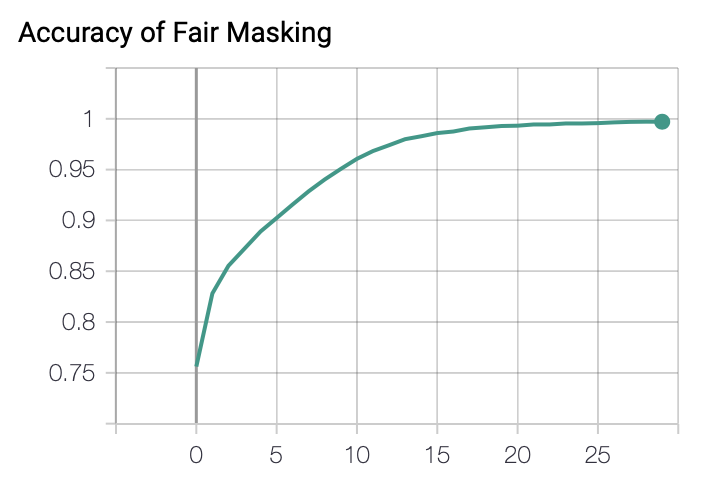
\includegraphics[width=0.4\textwidth]{figure/fairmasking-ac.png}
	\end{subfigure}
	\caption{Training loss and accuracy in gender classification for Fair Masked CNN.}
	\label{fig: fair masking cnn}
\end{figure}

\begin{itemize}
\item Training: final training accuracy and loss are 99.35$\%$ and 0.0001, respectively.  

\item Validation: final validation accuracy and loss are 85.42$\%$ and 0.0028, respectively.

\item UF for the validation set: unfairness parameter on the validation set is 0.0012.   
\end{itemize}

\subsubsection*{Performance with correlation-based dependence test}
Below are the plots of the unfairness and accuracy of fair-masked CNN on the validation set with different values of $T_c$.

\begin{figure}[H]
	\centering
	\begin{subfigure}
		\centering
		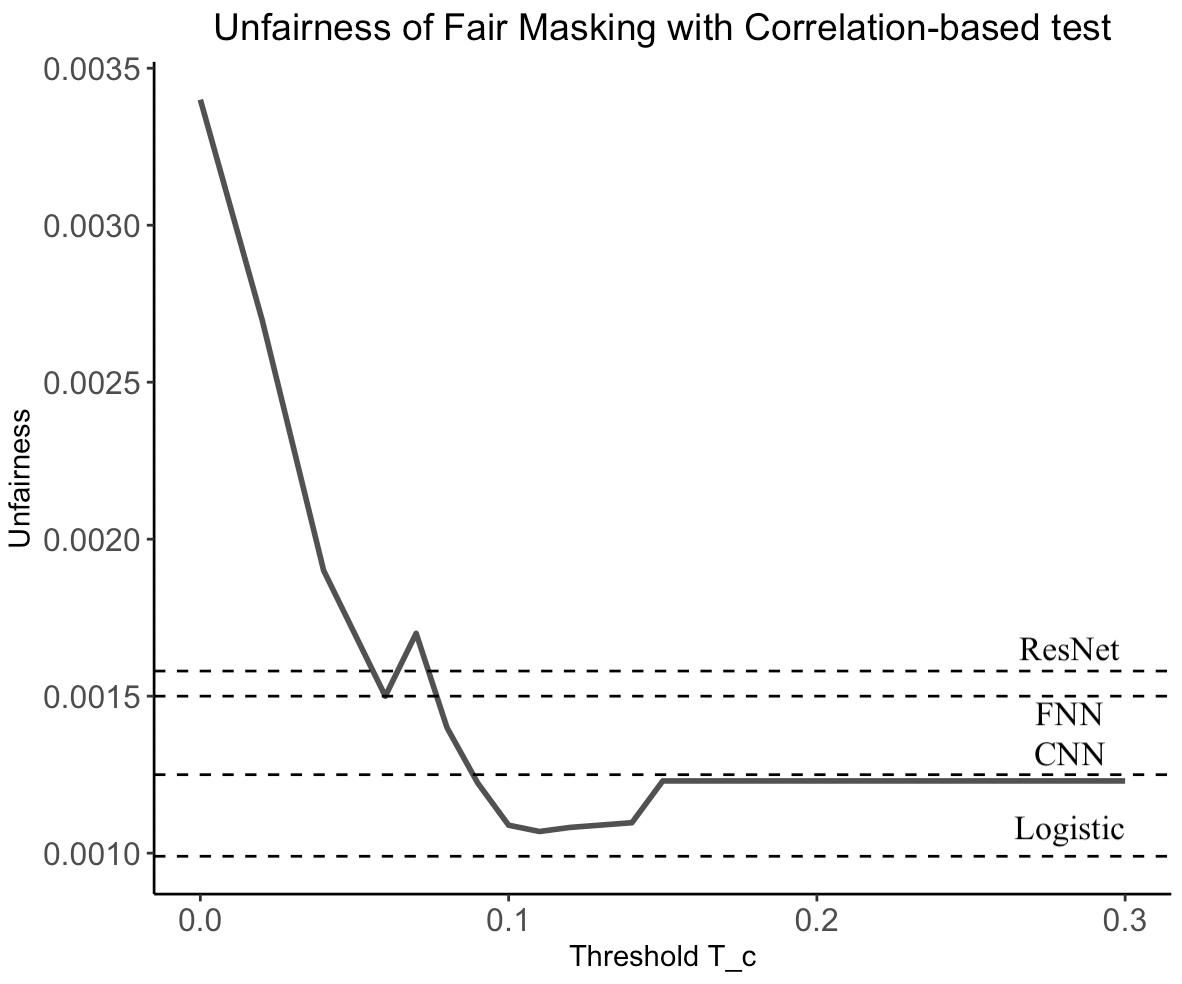
\includegraphics[width=0.4\textwidth]{figure/fairmasking-c-f.png}
	\end{subfigure}
	\quad
	\begin{subfigure}
		\centering
		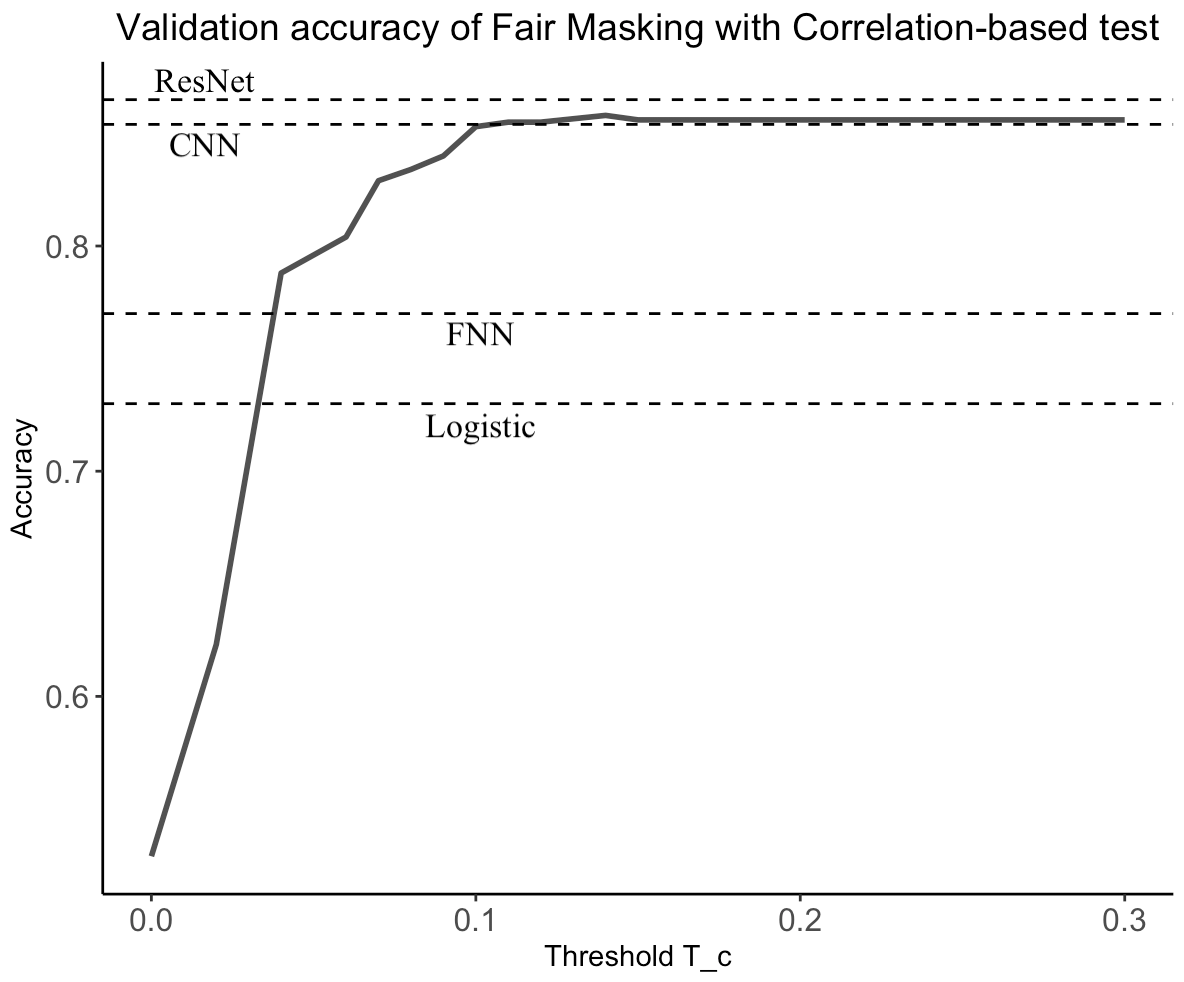
\includegraphics[width=0.4\textwidth]{figure/fairmasking-c-a.png}
	\end{subfigure}
	\caption{Unfairness and accuracy of Fair Masked CNN in gender prediction}
	\label{fig: fairmasking}
\end{figure}

The ranking of unfairness, from fairest to least fair, among all the baseline models is: logistic regression, CNN and FNN, and ResNet. Since our fair-masked CNN also adopts a CNN structure, we observe that when $T_c \rightarrow \infty$, in which none of the hidden features are masked out, the unfairness of the algorithm is very similar to that of CNN baseline.
\\ \\
We observe that the unfairness of the network decreases from around $T_c = 0.15$, where we select the first hidden feature from $\mathcal{H}$ to mask out, to  $T_c = 0.10$, where we select 6 out of 32 features. Afterwards, the unfairness increases as we select more hidden features. Notice that at the minimum of the curve, in which we select 6 features to mask out, the prediction accuracy is 85.31$\%$, which is similar to that of the CNN and ResNet baselines and significantly better than that of the logistic regression. However, the logistic regression model is a bit fairer than fair-masked CNN at $T_c = 0.1$, implying a fairness-performance trade-off involved in fair masking.
\\ \\ 
The result implies that, for fair masking with correlation test, a carefully chosen threshold will effectively mitigate the unfairness while doing little harm to the overall performance of the CNN in gender prediction.

\subsubsection*{Performance with logistic-regression-based dependence test}
Below are the plots of the unfairness and accuracy of fair-masked CNN on the validation set with different values of $T_l$.

\begin{figure}[H]
	\centering
	\begin{subfigure}
		\centering
		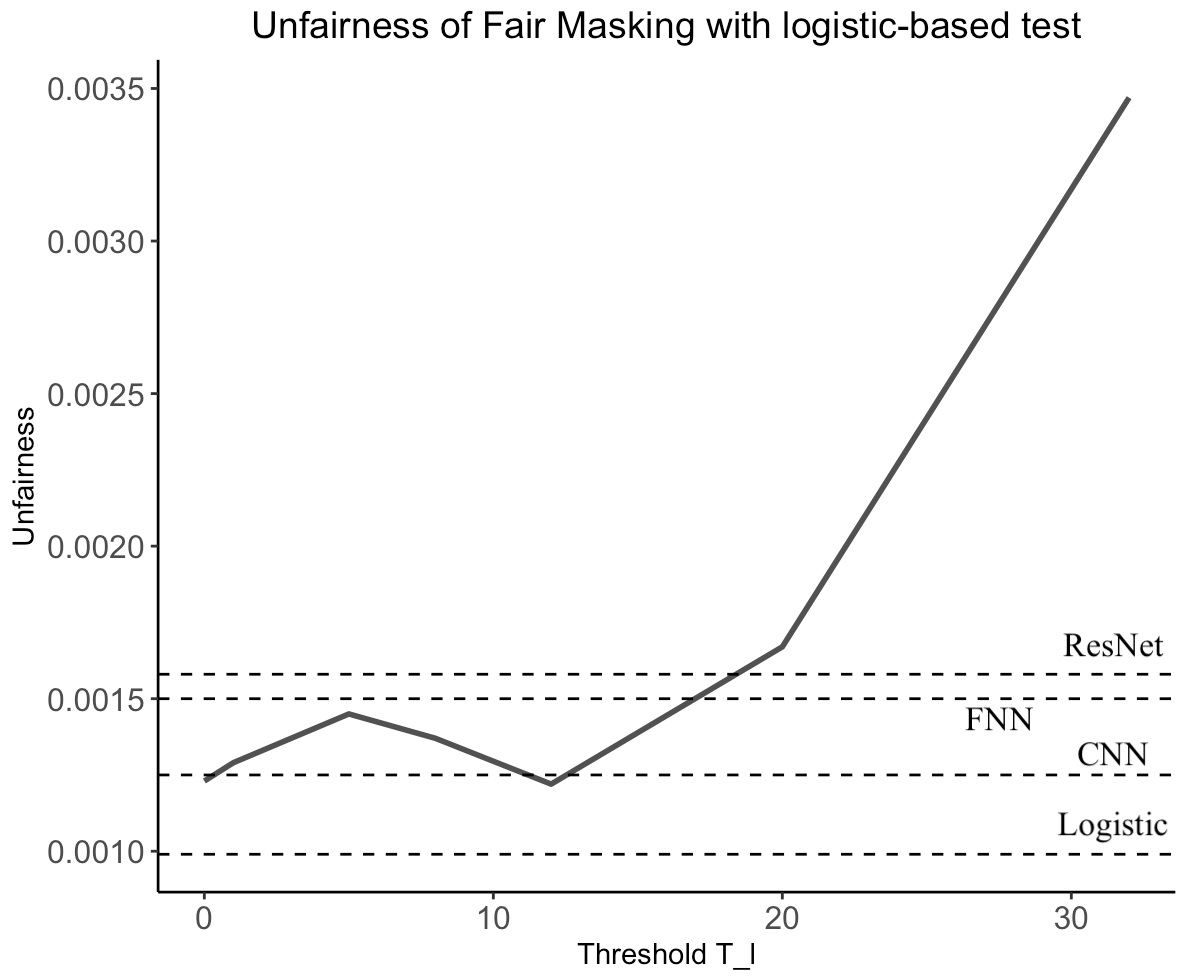
\includegraphics[width=0.4\textwidth]{figure/fairmasking-l-f.png}
	\end{subfigure}
	\quad
	\begin{subfigure}
		\centering
		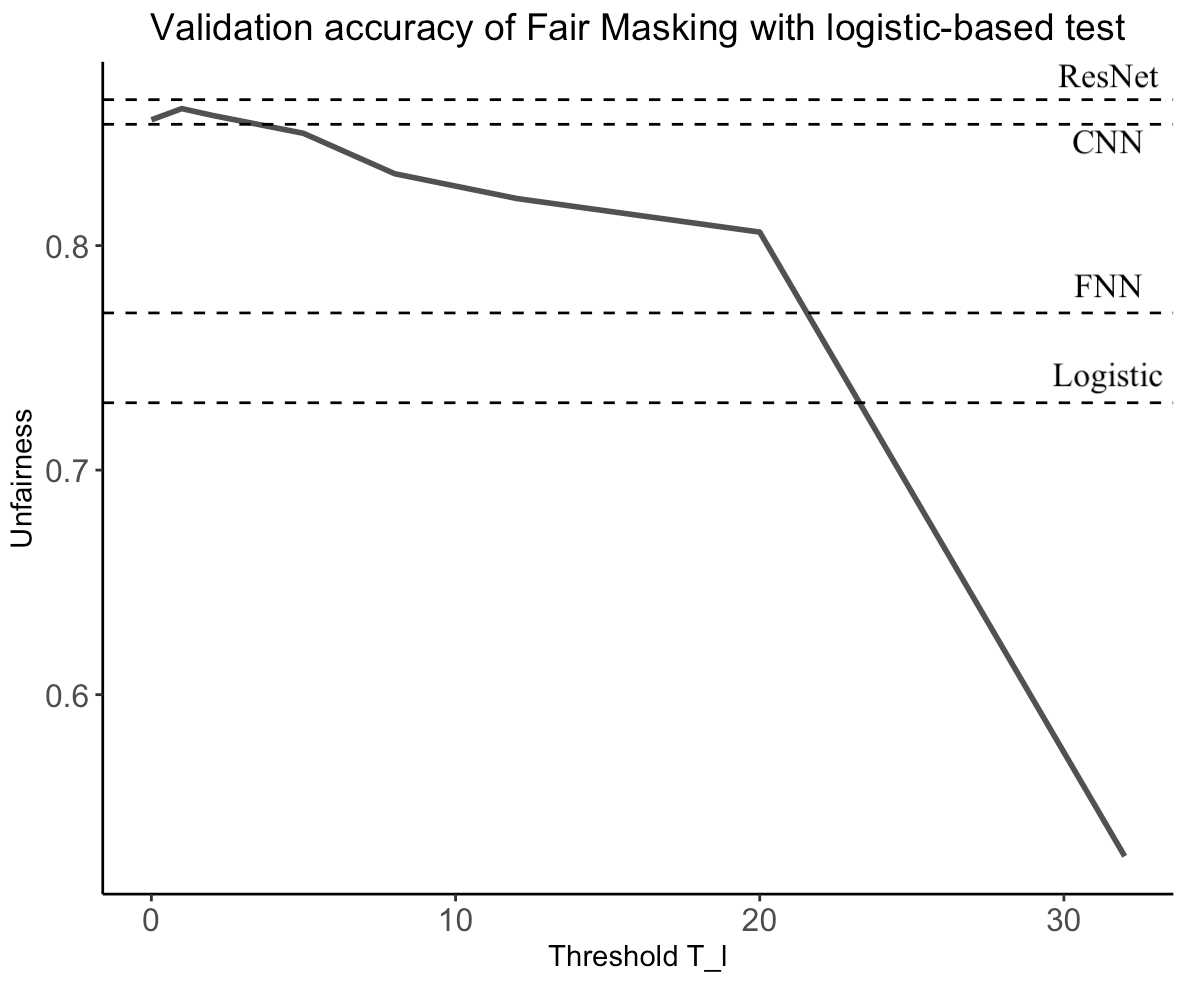
\includegraphics[width=0.4\textwidth]{figure/fairmasking-l-a.png}
	\end{subfigure}
	\caption{Unfairness and accuracy of Fair Masked CNN in gender prediction}
	\label{fig: fairmasking}
\end{figure}
Unfortunately, we observe that masking out several hidden features from $\mathcal{H}$ (no more than five) doesn't significantly affect the prediction accuracy on validation set, and, in fact, amplifies the algorithmic bias. We believe one potential reason for this failure is that the dependence test based on logistic regression is less effective than the correlation-based test, failing to select those that truly affect the bias of algorithm. We believe it is still possible to propose other novel dependence tests to select those features that affect algorithm bias.


\subsection{Novel approach (3) - Transfer Learning}

\begin{itemize}

\item Test: final test accuracy and loss are 62.81$\%$ and 0.0103, respectively.

\item UF for the validation set: unfairness parameter on the validation set is 0.0002.   
\end{itemize}

The overall test accuracy is significantly lower than the baselines' results, but above random chance.
\\
\\
While it inherently makes sense that accuracies for transfer learning would be below the baseline, these drops in accuracy are significant. We suggest some reasons why this may have occurred.
\begin{itemize}
\item The class imbalance of IMDb is extreme (see Figure 11 below), whereas the data that the model was trained on was fairly balanced.
\item There is significant mislabelling of data in IMDb. This is noted in \ref{imdb_data}, and certainly would have a negative effect on accuracy.
\item The FairFace images are cropped much more closely than the images in IMDb, which could impede classification accuracy. This can also be visually observed in the Data section.
\end{itemize}
\\
We can observe the distributions for gender and ethnicity across FairFace training, validation, and IMDB datasets below.
\begin{figure}[H]
	\centering
	\begin{subfigure}
		\centering
		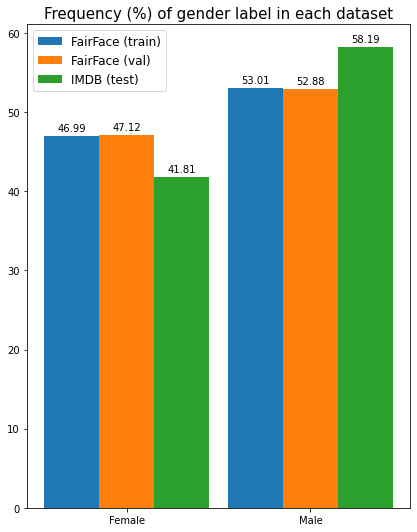
\includegraphics[width=0.32\textwidth]{figure/gender_hist.png}
	\end{subfigure}
	\quad
	\begin{subfigure}
		\centering
		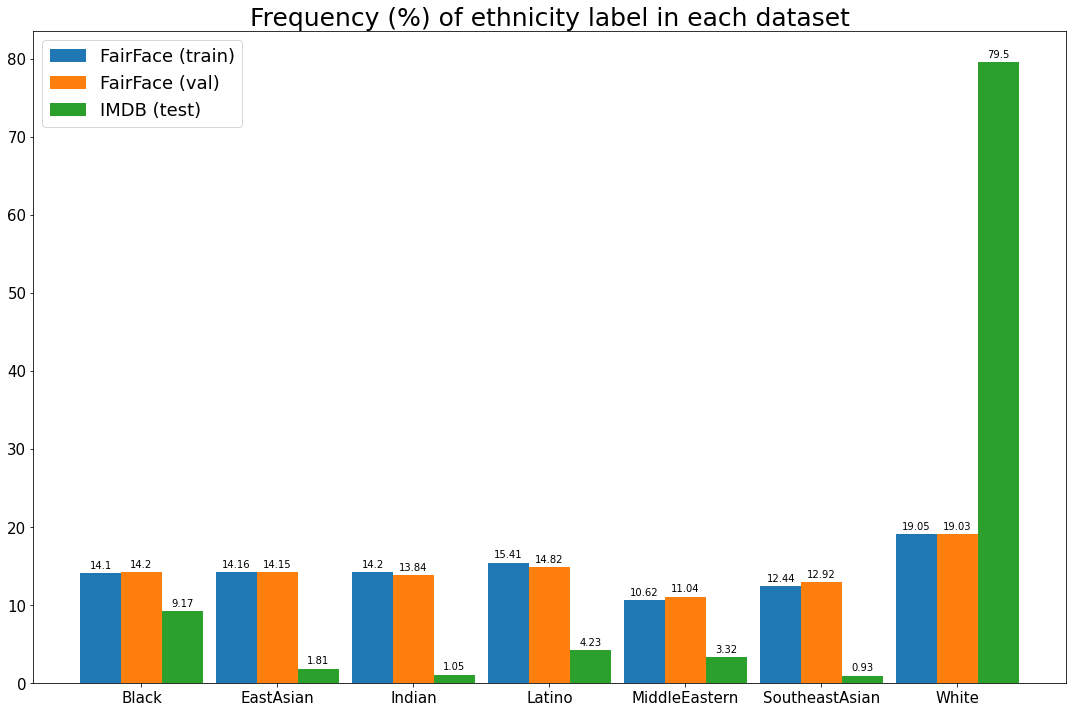
\includegraphics[width=0.62\textwidth]{figure/eth_hist.png}
	\end{subfigure}
	\caption{Distributions of gender and ethnicity across all datasets.}
	\label{fig: tran_learn}
\end{figure}
\\
\\
Interestingly, the unfairness measure for transfer learning was 0.0002, the lowest of all models. This means that the model was the most equally accurate (or inaccurate) across all ethnic groups. This may have to do with the fairness-performance trade-off discussed in the fair masking analysis.